\documentclass[11pt,fleqn, openany]{book} % Default font size and left-justified equations

%%%%%%%%%%%%%%%%%%%%%%%%%%%%%%%%%%%%%%%%%
% The Legrand Orange Book
% Structural Definitions File
% Version 2.1 (26/09/2018)
%
% Original author:
% Mathias Legrand (legrand.mathias@gmail.com) with modifications by:
% Vel (vel@latextemplates.com)
% 
% This file was downloaded from:
% http://www.LaTeXTemplates.com
%
% License:
% CC BY-NC-SA 3.0 (http://creativecommons.org/licenses/by-nc-sa/3.0/)
%
%%%%%%%%%%%%%%%%%%%%%%%%%%%%%%%%%%%%%%%%%

%----------------------------------------------------------------------------------------
%	VARIOUS REQUIRED PACKAGES AND CONFIGURATIONS
%----------------------------------------------------------------------------------------

\usepackage[table]{xcolor}

\usepackage{graphicx}
\usepackage{tabularx} % Required for including pictures
\usepackage{pgf,tikz,tkz-tab,eurosym,yhmath, stmaryrd}
\usepackage{pgfplots}
\usepackage{mathrsfs}
\usetikzlibrary{patterns}
\usetikzlibrary{trees}
\graphicspath{{../../Pictures/}}
\usepackage{multicol} 


\usepackage[english]{babel} % English language/hyphenation
\usepackage{icomma}
\usepackage{enumitem} % Customize lists
\setlist{nolistsep, nosep, nolistsep} % Reduce spacing between bullet points and numbered lists

\usepackage{booktabs} % Required for nicer horizontal rules in tables

 % Required for specifying colors by name


\definecolor{ocre}{RGB}{243,102,25} % Define the orange color used for highlighting throughout the book

\usepackage{listings}

\definecolor{codegreen}{rgb}{0,0.6,0}
\definecolor{codegray}{rgb}{0.5,0.5,0.5}
\definecolor{codepurple}{rgb}{0.58,0,0.82}
\definecolor{backcolour}{rgb}{0.95,0.95,0.92}

\lstdefinestyle{mystyle}{
    backgroundcolor=\color{backcolour},   
    commentstyle=\color{codegreen},
    keywordstyle=\color{magenta},
    numberstyle=\tiny\color{codegray},
    stringstyle=\color{codepurple},
    basicstyle=\ttfamily\footnotesize,
    breakatwhitespace=false,         
    breaklines=true,                 
    captionpos=b,                    
    keepspaces=true,                 
    numbers=left,                    
    numbersep=5pt,                  
    showspaces=false,                
    showstringspaces=false,
    showtabs=false,                  
    tabsize=2
}

\lstset{style=mystyle}

%----------------------------------------------------------------------------------------
% Paramétrage XSIM
%----------------------------------------------------------------------------------------

\usepackage[no-files]{xsim}


\DeclareExerciseEnvironmentTemplate{myex}{%
    \textbf{%
      \hypertarget{ex:\ExerciseID}{\sffamily{\ensuremath{\blacktriangleright}} Exercice \GetExerciseProperty{counter} \GetExerciseProperty{subtitle} --}
      \hyperlink{sol:\ExerciseID}{Voir le corrigé}%
    }\par
}{\par\smallskip}

\DeclareExerciseEnvironmentTemplate{mysol}{%
    \textbf{%
      \hypertarget{sol:\ExerciseID}{\sffamily{\ensuremath{\blacktriangleright}} Correction \GetExerciseProperty{counter} --}
      \hyperlink{ex:\ExerciseID}{Voir l'énoncé}%
    }\par
}{\par\medskip}

\xsimsetup{
  exercise/template = myex ,
  solution/template = mysol 
}

%Collection exercices

\DeclareExerciseTagging{topic}

\xsimsetup{collect}

%----------------------------------------------------------------------------------------
% SYMBOLES
%----------------------------------------------------------------------------------------

\newcommand\imCMsym[4][\mathord]{%
  \DeclareFontFamily{U} {#2}{}
  \DeclareFontShape{U}{#2}{m}{n}{
    <-6> #25
    <6-7> #26
    <7-8> #27
    <8-9> #28
    <9-10> #29
    <10-12> #210
    <12-> #212}{}
  \DeclareSymbolFont{CM#2} {U} {#2}{m}{n}
  \DeclareMathSymbol{#4}{#1}{CM#2}{#3}
}
\newcommand\alsoimCMsym[4][\mathord]{\DeclareMathSymbol{#4}{#1}{CM#2}{#3}}

\imCMsym{cmmi}{124}{\CMjmath}

\newcommand{\Oij}{(O\,;\,\vec{\imath}\,,\, \vec{\CMjmath} )}
\newcommand{\Oijk}{(O\,;\,\vec{\imath}\,,\, \vec{\CMjmath}\,,\,\vec{k})}

\newcommand\e{\mathrm{e}}
\newcommand\R{\mathbb{R}}
\newcommand\N{\mathbb{N}}


%----------------------------------------------------------------------------------------
%	MARGINS
%----------------------------------------------------------------------------------------

\usepackage{geometry} % Required for adjusting page dimensions and margins

\geometry{
	paper=a4paper, % Paper size, change to letterpaper for US letter size
	top=3cm, % Top margin
	bottom=3cm, % Bottom margin
	left=2cm, % Left margin
	right=2cm, % Right margin
	headheight=14pt, % Header height
	footskip=1.4cm, % Space from the bottom margin to the baseline of the footer
	headsep=10pt, % Space from the top margin to the baseline of the header
	%showframe, % Uncomment to show how the type block is set on the page
}

\setlength{\parindent}{0pt}
\parskip=5pt



%----------------------------------------------------------------------------------------
%	FONTS
%----------------------------------------------------------------------------------------

\usepackage{avant} % Use the Avantgarde font for headings
\usepackage{times} % Use the Times font for headings
\usepackage{mathptmx} % Use the Adobe Times Roman as the default text font together with math symbols from the Sym­bol, Chancery and Com­puter Modern fonts

%\usepackage{microtype} % Slightly tweak font spacing for aesthetics
%\usepackage[utf8]{inputenc} % Required for including letters with accents
\usepackage[T1]{fontenc} % Use 8-bit encoding that has 256 glyphs

%----------------------------------------------------------------------------------------
%	BIBLIOGRAPHY AND INDEX
%----------------------------------------------------------------------------------------

\usepackage[style=numeric,citestyle=numeric,sorting=nyt,sortcites=true,autopunct=true,babel=hyphen,hyperref=true,abbreviate=false,backref=true,backend=biber]{biblatex}
\addbibresource{bibliography.bib} % BibTeX bibliography file
\defbibheading{bibempty}{}

\usepackage{calc} % For simpler calculation - used for spacing the index letter headings correctly
\usepackage{makeidx} % Required to make an index
\makeindex % Tells LaTeX to create the files required for indexing

%----------------------------------------------------------------------------------------
%	MAIN TABLE OF CONTENTS
%----------------------------------------------------------------------------------------

\usepackage{titletoc} % Required for manipulating the table of contents

\contentsmargin{0cm} % Removes the default margin

% Part text styling (this is mostly taken care of in the PART HEADINGS section of this file)
\titlecontents{part}
	[0cm] % Left indentation
	{\addvspace{20pt}\bfseries} % Spacing and font options for parts
	{}
	{}
	{}

% Chapter text styling
\titlecontents{chapter}
	[1.25cm] % Left indentation
	{\addvspace{12pt}\large\sffamily\bfseries} % Spacing and font options for chapters
	{\color{ocre!60}\contentslabel[\Large\thecontentslabel]{1.25cm}\color{ocre}} % Formatting of numbered sections of this type
	{\color{ocre}} % Formatting of numberless sections of this type
	{\color{ocre!60}\normalsize\;\titlerule*[.5pc]{.}\;\thecontentspage} % Formatting of the filler to the right of the heading and the page number

% Section text styling
\titlecontents{section}
	[1.25cm] % Left indentation
	{\addvspace{3pt}\sffamily\bfseries} % Spacing and font options for sections
	{\contentslabel[\thecontentslabel]{1.25cm}} % Formatting of numbered sections of this type
	{} % Formatting of numberless sections of this type
	{\hfill\color{black}\thecontentspage} % Formatting of the filler to the right of the heading and the page number

% Subsection text styling
\titlecontents{subsection}
	[1.25cm] % Left indentation
	{\addvspace{1pt}\sffamily\small} % Spacing and font options for subsections
	{\contentslabel[\thecontentslabel]{1.25cm}} % Formatting of numbered sections of this type
	{} % Formatting of numberless sections of this type
	{\ \titlerule*[.5pc]{.}\;\thecontentspage} % Formatting of the filler to the right of the heading and the page number

% Figure text styling
\titlecontents{figure}
	[1.25cm] % Left indentation
	{\addvspace{1pt}\sffamily\small} % Spacing and font options for figures
	{\thecontentslabel\hspace*{1em}} % Formatting of numbered sections of this type
	{} % Formatting of numberless sections of this type
	{\ \titlerule*[.5pc]{.}\;\thecontentspage} % Formatting of the filler to the right of the heading and the page number

% Table text styling
\titlecontents{table}
	[1.25cm] % Left indentation
	{\addvspace{1pt}\sffamily\small} % Spacing and font options for tables
	{\thecontentslabel\hspace*{1em}} % Formatting of numbered sections of this type
	{} % Formatting of numberless sections of this type
	{\ \titlerule*[.5pc]{.}\;\thecontentspage} % Formatting of the filler to the right of the heading and the page number

%----------------------------------------------------------------------------------------
%	MINI TABLE OF CONTENTS IN PART HEADS
%----------------------------------------------------------------------------------------

% Chapter text styling
\titlecontents{lchapter}
	[0em] % Left indentation
	{\addvspace{15pt}\large\sffamily\bfseries} % Spacing and font options for chapters
	{\color{ocre}\contentslabel[\Large\thecontentslabel]{1.25cm}\color{ocre}} % Chapter number
	{}  
	{\color{ocre}\normalsize\sffamily\bfseries\;\titlerule*[.5pc]{.}\;\thecontentspage} % Page number

% Section text styling
\titlecontents{lsection}
	[0em] % Left indentation
	{\sffamily\small} % Spacing and font options for sections
	{\contentslabel[\thecontentslabel]{1.25cm}} % Section number
	{}
	{}

% Subsection text styling (note these aren't shown by default, display them by searchings this file for tocdepth and reading the commented text)
\titlecontents{lsubsection}
	[.5em] % Left indentation
	{\sffamily\footnotesize} % Spacing and font options for subsections
	{\contentslabel[\thecontentslabel]{1.25cm}}
	{}
	{}

%----------------------------------------------------------------------------------------
%	HEADERS AND FOOTERS
%----------------------------------------------------------------------------------------


\usepackage{fancyhdr} % Required for header and footer configuration

\pagestyle{fancy}
\renewcommand{\chaptermark}[1]{\markboth{\sffamily\normalsize\bfseries\ \thechapter.\ #1}{}} % Chapter text font settings
\renewcommand{\sectionmark}[1]{\markright{\sffamily\normalsize\thesection\hspace{5pt}#1}{}} % Section text font settings
\fancyhf{} \fancyhead[LE,RO]{\sffamily\normalsize\thepage} % Font setting for the page number in the header
\fancyhead[LO]{\rightmark} % Print the nearest section name on the left side of odd pages
\fancyhead[RE]{\leftmark} % Print the current chapter name on the right side of even pages

\fancyfoot[L]{Jason LAPEYRONNIE}
\fancyfoot[R]{\href{http://mathoutils.fr}{http://mathoutils.fr}} % Uncomment to include a footer

\renewcommand{\headrulewidth}{0.5pt} % Thickness of the rule under the header
\renewcommand{\footrulewidth}{0.5pt} % Thickness of the rule under the header

\fancypagestyle{plain}{% Style for when a plain pagestyle is specified
	\fancyhead{}\renewcommand{\headrulewidth}{0pt}%
}

% Removes the header from odd empty pages at the end of chapters
\makeatletter
\renewcommand{\cleardoublepage}{
\clearpage\ifodd\c@page\else
\hbox{}
\vspace*{\fill}
\thispagestyle{empty}
\newpage
\fi}

%----------------------------------------------------------------------------------------
%	THEOREM STYLES
%----------------------------------------------------------------------------------------

\usepackage{amsmath,amsfonts,amssymb,amsthm} % For math equations, theorems, symbols, etc

\newcommand{\intoo}[2]{\mathopen{]}#1\,;#2\mathclose{[}}
\newcommand{\ud}{\mathop{\mathrm{{}d}}\mathopen{}}
\newcommand{\intff}[2]{\mathopen{[}#1\,;#2\mathclose{]}}
\renewcommand{\qedsymbol}{$\blacksquare$}
\newtheorem{notation}{Notation}[section]

% Boxed/framed environments
\newtheoremstyle{ocrenumbox}% Theorem style name
{0pt}% Space above
{0pt}% Space below
{\normalfont}% Body font
{}% Indent amount
{\small\bf\sffamily\color{ocre}}% Theorem head font
{\;:\;}% Punctuation after theorem head
{0.25em}% Space after theorem head
{\small\sffamily\color{ocre}\thmname{#1}\nobreakspace\thmnumber{\@ifnotempty{#1}{}\@upn{#2}}% Theorem text (e.g. Theorem 2.1)
\thmnote{\nobreakspace\the\thm@notefont\sffamily\bfseries\color{black}---\nobreakspace#3}} % Optional theorem note

\newtheoremstyle{blacknumex}% Theorem style name
{5pt}% Space above
{10pt}% Space below
{\normalfont}% Body font
{} % Indent amount
{\small\bf\sffamily}% Theorem head font
{\;:\;}% Punctuation after theorem head
{0.25em}% Space after theorem head
{\small\sffamily{\tiny\ensuremath{\blacksquare}}\nobreakspace\thmname{#1}\nobreakspace\thmnumber{\@ifnotempty{#1}{}\@upn{#2}}% Theorem text (e.g. Theorem 2.1)
\thmnote{\nobreakspace\the\thm@notefont\sffamily\bfseries---\nobreakspace#3}}% Optional theorem note

\newtheoremstyle{blacknumexo}% Theorem style name
{15pt}% Space above
{10pt}% Space below
{\normalfont}% Body font
{} % Indent amount
{\small\bf\sffamily}% Theorem head font
{}% Punctuation after theorem head
{0.5em}% Space after theorem head
{\small\sffamily{\ensuremath{\blacktriangleright}}\nobreakspace\thmname{#1}\nobreakspace\thmnumber{\@ifnotempty{#1}{}\@upn{#2}}% Theorem text (e.g. Theorem 2.1)
\thmnote{\nobreakspace\the\thm@notefont\sffamily\bfseries---\nobreakspace#3} \\}% Optional theorem note



\newtheoremstyle{blacknumbox} % Theorem style name
{0pt}% Space above
{5pt}% Space below
{}% Body font
{}% Indent amount
{\large\bf\sffamily}% Theorem head font
{\;:\;}% Punctuation after theorem head
{0.25em}% Space after theorem head
{\small\sffamily\thmname{#1}\nobreakspace\thmnumber{\@ifnotempty{#1}{}\@upn{#2}}% Theorem text (e.g. Theorem 2.1)
\thmnote{\nobreakspace\the\thm@notefont\sffamily\bfseries---\nobreakspace#3}}% Optional theorem note

% Non-boxed/non-framed environments
\newtheoremstyle{ocrenum}% Theorem style name
{5pt}% Space above
{5pt}% Space below
{\normalfont}% Body font
{}% Indent amount
{\small\bf\sffamily\color{ocre}}% Theorem head font
{\;:\;}% Punctuation after theorem head
{0.25em}% Space after theorem head
{\small\sffamily\color{ocre}\thmname{#1}\nobreakspace\thmnumber{\@ifnotempty{#1}{}\@upn{#2}}% Theorem text (e.g. Theorem 2.1)
\thmnote{\nobreakspace\the\thm@notefont\sffamily\bfseries\color{black}---\nobreakspace#3}} % Optional theorem note
\makeatother

% Defines the theorem text style for each type of theorem to one of the three styles above
\newcounter{dummy} 
\newcounter{thm}
\newcounter{correction}
\newcounter{qst}
\theoremstyle{ocrenumbox}
\newtheorem{theoremeT}[dummy]{Théorème}
\newtheorem{exerciseT}{Propriété}
\newtheorem{principeT}{Principe}
\theoremstyle{blacknumex}
\newtheorem{exampleT}{Exemple}
\theoremstyle{blacknumexo}
\newtheorem{exo}[thm]{Exercice}
\newtheorem{corr}[correction]{Correction}
\newtheorem{quest}[qst]{Question}
\theoremstyle{blacknumbox}
\newtheorem{vocabulary}{Vocabulary}[section]
\newtheorem{definitionT}{Définition}
\newtheorem{corollaryT}[dummy]{Corollary}
\theoremstyle{ocrenum}
\newtheorem{proofT}[dummy]{Démonstration}


%----------------------------------------------------------------------------------------
%	DEFINITION OF COLORED BOXES
%----------------------------------------------------------------------------------------

\RequirePackage[framemethod=default]{mdframed} % Required for creating the theorem, definition, exercise and corollary boxes

% Theorem box
\newmdenv[skipabove=7pt,
skipbelow=7pt,
backgroundcolor=black!5,
linecolor=ocre,
innerleftmargin=5pt,
innerrightmargin=5pt,
innertopmargin=10pt,
leftmargin=0cm,
rightmargin=0cm,
innerbottommargin=5pt]{tBox}

%Proposition box	  
\newmdenv[skipabove=7pt,
skipbelow=7pt,
rightline=false,
leftline=true,
topline=false,
bottomline=false,
backgroundcolor=ocre!10,
linecolor=ocre,
innerleftmargin=5pt,
innerrightmargin=5pt,
innertopmargin=10pt,
innerbottommargin=3pt,
leftmargin=0cm,
rightmargin=0cm,
linewidth=4pt]{eBox}	

% Definition box
\newmdenv[skipabove=7pt,
backgroundcolor=ocre!4,
skipbelow=7pt,
rightline=false,
leftline=true,
topline=false,
bottomline=false,
linecolor=ocre,
innerleftmargin=5pt,
innerrightmargin=5pt,
innertopmargin=10pt,
leftmargin=0cm,
rightmargin=0cm,
linewidth=4pt,
innerbottommargin=5pt]{dBox}	

% Corollary box
\newmdenv[skipabove=7pt,
skipbelow=7pt,
rightline=false,
leftline=true,
topline=false,
bottomline=false,
linecolor=gray,
backgroundcolor=black!5,
innerleftmargin=5pt,
innerrightmargin=5pt,
innertopmargin=5pt,
leftmargin=0cm,
rightmargin=0cm,
linewidth=4pt,
innerbottommargin=5pt]{cBox}

\newmdenv[skipabove=7pt,
skipbelow=7pt,
backgroundcolor=black!5,
innerleftmargin=5pt,
topline=false,
bottomline=false,
rightline=false,
leftline=false,
innerrightmargin=5pt,
innertopmargin=5pt,
leftmargin=0cm,
rightmargin=0cm,
innerbottommargin=5pt]{xBox}

% Creates an environment for each type of theorem and assigns it a theorem text style from the "Theorem Styles" section above and a colored box from above
\newenvironment{theorem}{\begin{tBox}\begin{theoremeT}}{\end{theoremeT}\end{tBox}}

\newenvironment{exo2}{\noindent \begin{exo}\item\relax \noindent \begin{eBox}\item\relax}{\end{eBox}\end{exo}}


\newenvironment{proposition}{\begin{eBox}\begin{exerciseT}}{\hfill{\color{ocre}}\end{exerciseT}\end{eBox}}		

\newenvironment{principe}{\begin{eBox}\begin{principeT}}{\hfill{\color{ocre}}\end{principeT}\end{eBox}}	
		  
\newenvironment{definition}{\begin{dBox}\begin{definitionT}}{\end{definitionT}\end{dBox}}	

\newenvironment{example}{\begin{xBox}\begin{exampleT}}{\hfill{\tiny\ensuremath{\blacksquare}}\end{exampleT}\end{xBox}}

\newenvironment{demonstration}{\begin{proofT}}{\hfill{\tiny\ensuremath{\square}}\end{proofT}}		
\newenvironment{corollary}{\begin{cBox}\begin{corollaryT}}{\end{corollaryT}\end{cBox}}	

%----------------------------------------------------------------------------------------
%	REMARK ENVIRONMENT
%----------------------------------------------------------------------------------------

\newenvironment{remark}{\par\vspace{5pt}\small % Vertical white space above the remark and smaller font size
\begin{list}{}{
\leftmargin=25pt % Indentation on the left
\rightmargin=15pt}\item\ignorespaces % Indentation on the right
\makebox[-2.5pt]{
\begin{tikzpicture}[overlay]
\node[draw=ocre!60,line width=1pt,circle,fill=ocre!25,font=\sffamily\bfseries,inner sep=2pt,outer sep=0pt] at (-15pt,0pt){\textcolor{ocre}{R}};\end{tikzpicture}} % Orange R in a circle
\advance\baselineskip -1pt}{\end{list}\vskip5pt} % Tighter line spacing and white space after remark

%----------------------------------------------------------------------------------------
%	SECTION NUMBERING IN THE MARGIN
%----------------------------------------------------------------------------------------

\makeatletter
\renewcommand{\@seccntformat}[1]{\llap{\textcolor{ocre}{\csname the#1\endcsname}\hspace{1em}}}                    
\renewcommand{\section}{\@startsection{section}{1}{\z@}
{-4ex \@plus -1ex \@minus -.4ex}
{1ex \@plus.2ex }
{\normalfont\LARGE\sffamily\bfseries}}
\renewcommand{\subsection}{\@startsection {subsection}{2}{\z@}
{-3ex \@plus -0.1ex \@minus -.4ex}
{0.5ex \@plus.2ex }
{\normalfont\sffamily\bfseries}}
\renewcommand{\subsubsection}{\@startsection {subsubsection}{3}{\z@}
{-2ex \@plus -0.1ex \@minus -.2ex}
{.2ex \@plus.2ex }
{\normalfont\small\sffamily\bfseries}}                        
\renewcommand\paragraph{\@startsection{paragraph}{4}{\z@}
{-2ex \@plus-.2ex \@minus .2ex}
{.1ex}
{\normalfont\small\sffamily\bfseries}}

%----------------------------------------------------------------------------------------
%	PART HEADINGS
%----------------------------------------------------------------------------------------

% Numbered part in the table of contents
\newcommand{\@mypartnumtocformat}[2]{%
	\setlength\fboxsep{0pt}%
	\noindent\colorbox{ocre!20}{\strut\parbox[c][.7cm]{\ecart}{\color{ocre!70}\Large\sffamily\bfseries\centering#1}}\hskip\esp\colorbox{ocre!40}{\strut\parbox[c][.7cm]{\linewidth-\ecart-\esp}{\Large\sffamily\centering#2}}%
}

% Unnumbered part in the table of contents
\newcommand{\@myparttocformat}[1]{%
	\setlength\fboxsep{0pt}%
	\noindent\colorbox{ocre!40}{\strut\parbox[c][.7cm]{\linewidth}{\Large\sffamily\centering#1}}%
}

\newlength\esp
\setlength\esp{4pt}
\newlength\ecart
\setlength\ecart{1.2cm-\esp}
\newcommand{\thepartimage}{}%
\newcommand{\partimage}[1]{\renewcommand{\thepartimage}{#1}}%
\def\@part[#1]#2{%
\ifnum \c@secnumdepth >-2\relax%
\refstepcounter{part}%
\addcontentsline{toc}{part}{\texorpdfstring{\protect\@mypartnumtocformat{\thepart}{#1}}{\partname~\thepart\ ---\ #1}}
\else%
\addcontentsline{toc}{part}{\texorpdfstring{\protect\@myparttocformat{#1}}{#1}}%
\fi%
\startcontents%
\markboth{}{}%
{\thispagestyle{empty}%
\begin{tikzpicture}[remember picture,overlay]%
\node at (current page.north west){\begin{tikzpicture}[remember picture,overlay]%	
\fill[ocre!20](0cm,0cm) rectangle (\paperwidth,-\paperheight);
\node[anchor=north] at (4cm,-3.25cm){\color{ocre!40}\fontsize{220}{100}\sffamily\bfseries\thepart}; 
\node[anchor=south east] at (\paperwidth-1cm,-\paperheight+1cm){\parbox[t][][t]{8.5cm}{
\printcontents{l}{0}{\setcounter{tocdepth}{1}}% The depth to which the Part mini table of contents displays headings; 0 for chapters only, 1 for chapters and sections and 2 for chapters, sections and subsections
}};
\node[anchor=north east] at (\paperwidth-1.5cm,-3.25cm){\parbox[t][][t]{15cm}{\strut\raggedleft\color{white}\fontsize{30}{30}\sffamily\bfseries#2}};
\end{tikzpicture}};
\end{tikzpicture}}%
\@endpart}
\def\@spart#1{%
\startcontents%
\phantomsection
{\thispagestyle{empty}%
\begin{tikzpicture}[remember picture,overlay]%
\node at (current page.north west){\begin{tikzpicture}[remember picture,overlay]%	
\fill[ocre!20](0cm,0cm) rectangle (\paperwidth,-\paperheight);
\node[anchor=north east] at (\paperwidth-1.5cm,-3.25cm){\parbox[t][][t]{15cm}{\strut\raggedleft\color{white}\fontsize{30}{30}\sffamily\bfseries#1}};
\end{tikzpicture}};
\end{tikzpicture}}
\addcontentsline{toc}{part}{\texorpdfstring{%
\setlength\fboxsep{0pt}%
\noindent\protect\colorbox{ocre!40}{\strut\protect\parbox[c][.7cm]{\linewidth}{\Large\sffamily\protect\centering #1\quad\mbox{}}}}{#1}}%
\@endpart}
\def\@endpart{\vfil\newpage
\if@twoside
\if@openright
\null
\thispagestyle{empty}%
\newpage
\fi
\fi
\if@tempswa
\twocolumn
\fi}

%----------------------------------------------------------------------------------------
%	CHAPTER HEADINGS
%----------------------------------------------------------------------------------------

% A switch to conditionally include a picture, implemented by Christian Hupfer
\newif\ifusechapterimage
\usechapterimagetrue
\newcommand{\thechapterimage}{}%
\newcommand{\chapterimage}[1]{\ifusechapterimage\renewcommand{\thechapterimage}{#1}\fi}%
\newcommand{\autodot}{.}
\def\@makechapterhead#1{%
{\parindent \z@ \raggedright \normalfont
\ifnum \c@secnumdepth >\m@ne
\if@mainmatter
\begin{tikzpicture}[remember picture,overlay]
\node at (current page.north west)
{\begin{tikzpicture}[remember picture,overlay]
\node[anchor=north west,inner sep=0pt] at (0,0) {\ifusechapterimage\includegraphics[width=\paperwidth]{\thechapterimage}\fi};
\draw[anchor=west] (\Gm@lmargin,-3cm) node [line width=2pt,rounded corners=15pt,draw=ocre,fill=white,fill opacity=0.5,inner sep=15pt]{\strut\makebox[22cm]{}};
\draw[anchor=west] (\Gm@lmargin+.3cm,-3cm) node {\huge\sffamily\bfseries\color{black}\thechapter\autodot~#1\strut};
\end{tikzpicture}};
\end{tikzpicture}
\else
\begin{tikzpicture}[remember picture,overlay]
\node at (current page.north west)
{\begin{tikzpicture}[remember picture,overlay]
\node[anchor=north west,inner sep=0pt] at (0,0) {\ifusechapterimage\includegraphics[width=\paperwidth]{\thechapterimage}\fi};
\draw[anchor=west] (\Gm@lmargin,-3cm) node [line width=2pt,rounded corners=15pt,draw=ocre,fill=white,fill opacity=0.5,inner sep=15pt]{\strut\makebox[22cm]{}};
\draw[anchor=west] (\Gm@lmargin+.3cm,-3cm) node {\huge\sffamily\bfseries\color{black}#1\strut};
\end{tikzpicture}};
\end{tikzpicture}
\fi\fi\par\vspace*{50\p@}}}

%-------------------------------------------

\def\@makeschapterhead#1{%
\begin{tikzpicture}[remember picture,overlay]
\node at (current page.north west)
{\begin{tikzpicture}[remember picture,overlay]
\node[anchor=north west,inner sep=0pt] at (0,0) {\ifusechapterimage\includegraphics[width=\paperwidth]{\thechapterimage}\fi};
\draw[anchor=west] (\Gm@lmargin,-3cm) node [line width=2pt,rounded corners=15pt,draw=ocre,fill=white,fill opacity=0.5,inner sep=15pt]{\strut\makebox[22cm]{}};
\draw[anchor=west] (\Gm@lmargin+.3cm,-3cm) node {\huge\sffamily\bfseries\color{black}#1\strut};
\end{tikzpicture}};
\end{tikzpicture}
\par\vspace*{50\p@}}
\makeatother

%----------------------------------------------------------------------------------------
%	LINKS
%----------------------------------------------------------------------------------------

\usepackage{hyperref}
\hypersetup{hidelinks,backref=true,pagebackref=true,hyperindex=true,colorlinks=false,breaklinks=true,urlcolor=ocre,bookmarks=true,bookmarksopen=false}

\usepackage{bookmark}
\bookmarksetup{
open,
numbered,
addtohook={%
\ifnum\bookmarkget{level}=0 % chapter
\bookmarksetup{bold}%
\fi
\ifnum\bookmarkget{level}=-1 % part
\bookmarksetup{color=ocre,bold}%
\fi
}
}

\renewcommand*\thesection{\arabic{section}}

\newcommand*{\coord}[3]{% 
  \ensuremath{\overrightarrow{#1}\, 
    \begin{pmatrix} 
      #2\\ 
      #3 
    \end{pmatrix}}}
    
  \newcommand*{\coordb}[2]{% 
  \ensuremath{ 
    \begin{pmatrix} 
      #1\\ 
      #2 
    \end{pmatrix}}}

\newcommand*{\coorde}[4]{% 
  \renewcommand{\arraystretch}{1}\ensuremath{\overrightarrow{#1}\, 
    \begin{pmatrix} 
      #2\\ 
      #3 \\
      #4
    \end{pmatrix}}}    
  \newcommand*{\coordbe}[3]{% 
 \renewcommand{\arraystretch}{1} \ensuremath{ 
    \begin{pmatrix} 
      #1\\ 
      #2 \\
      #3
    \end{pmatrix}}}  
    
\newcommand{\Card}{\mathrm{Card}}




\begin{document}

\chapterimage{../../Pictures/background}


\chapter{Cours : Loi binomiale}


\section{Succession d'épreuves indépendantes}



\begin{definition}[Succession d'épreuves]Soit $n$ un entier naturel. On considère $n$ épreuves aléatoires dont les univers sont respectivement $\Omega_1$, $\Omega_2$, ... , $\Omega_n$.

L'univers $\Omega$ de la succession de ces $n$ épreuves est le produit cartésien $\Omega_1 \times \Omega_2 \times \dots \times \Omega_n$.

Les issues de cette succession d'expériences sont les $n$-uplets $(i_1\, ;\, i_2\,;\,\dots\,;\,i_n)$ de $\Omega_1 \times \Omega_2 \times \dots \times \Omega_n$.\end{definition}

\begin{example}On lance 2 fois un dé à 6 faces, numérotées de $1$ à $6$ et on regarde le numéro obtenu. L'univers de cette expérience est $\{1;2;3;4;5;6\}^2$. L'issue $(1\,;\,3)$ signifie que l'on a obtenu 1 au premier lancer et 3 au deuxième.\end{example}

\begin{definition}[Indépendance mutuelle]Soit $n$ un entier naturel. On considère $n$ épreuves aléatoires dont les univers sont respectivement $\Omega_1$, $\Omega_2$, ... , $\Omega_n$, de lois respectives $\mathbb{P}_1$, $\mathbb{P}_2$, ... , $\mathbb{P}_n$.

Les épreuves sont dites mutuellement indépendantes (ou tout simplement indépendantes) si, pour toute issue $(i_1,i_2,...,i_n)$ de $\Omega_1 \times \Omega_2 \times \dots \times \Omega_n$, on a
\[ \mathbb{P}((i_1,i_2,...,i_n))=\mathbb{P}_1(i_1) \times \mathbb{P}_2(i_2) \times \dots \times \mathbb{P}_n(i_n).\]
Autrement dit, la probabilité d'une issue est égale au produit des probabilités de chacune des composantes $i_1$, $i_2$, ..., $i_n$.\end{definition}

\begin{example}M. Lapeyronnie a décidé de faire un petit contrôle surprise à ses élèves. Il place les noms des élèves de la classe dans une urne et une liste d'exercices dans une autre. 
\begin{itemize}
\item Il y a 29 élèves dans la classe. Parmi eux, 12 suivent l'option Maths expertes ;
\item L'urne des exercices en contient 40 : 20 sur les fonctions, 15 sur les suites et 5 sur la géométrie.
\end{itemize}
M. Lapeyronnie tire alors simultanément, de manière indépendante, un nom d'élève et un exercice.

\begin{itemize}
\item La probabilité qu'il s'agisse d'un élève suivant l'option Maths expertes est de $\dfrac{12}{29}$ ;
\vskip10pt
\item La probabilité de tirer un exercice de géométrie est de $\dfrac{5}{40}=\dfrac{1}{8}$ ;
\vskip10pt
\item La probabilité qu'un élève suivant l'option Maths Expertes soit envoyé au tableau faire un exercice de géométrie est donc de $\dfrac{12}{29} \times \dfrac{1}{8} = \dfrac{3}{58}$.
\end{itemize}
\end{example}

Si l'on essaie de représenter une succession de $n$ épreuves indépendantes sous la forme d'un arbre de probabilités, on place alors toujours le même sous-arbre à chaque noeud d'un étage fixé. De plus, cet arbre peut être construit "dans un sens comme dans l'autre".
\newpage
\begin{example}Les arbres suivants traduisent la succession des deux épreuves précédentes. 


\noindent\begin{minipage}{0.49\linewidth}
\tikzstyle{level 1}=[level distance=3.5cm, sibling distance=5cm]
\tikzstyle{level 2}=[level distance=3.5cm, sibling distance=2cm]
\tikzstyle{level 3}=[level distance=3.5cm, sibling distance=0.3cm]

% Define styles for bags and leafs
\tikzstyle{bag} = []
\tikzstyle{end} = [circle, minimum width=3pt,fill, inner sep=0pt]


\begin{center}
\begin{tikzpicture}[scale=0.8,grow=right,sloped]
\node[bag] { }
	child {
        node[bag] {Maths Exp.} 
        child {
                node[bag] {Géométrie}
                edge from parent node[below] {$1/8$}
            }
        child {
               node[bag] {Suites}
               edge from parent node[above] {$3/8$}
            }
        child {
                node[bag] {Fonctions}
                edge from parent node[above] {$1/2$}
            }
            edge from parent node[above] {$12/29$} 
    }
	child {
        node[bag] {Pas Maths Exp.} 
        child {
                node[bag] {Géométrie}
                edge from parent node[below] {$1/8$}
            }
        child {
               node[bag] {Suites}
               edge from parent node[above] {$3/8$}
            }
        child {
                node[bag] {Fonctions}
                edge from parent node[above] {$1/2$}
            }
            edge from parent node[above] {$17/29$}  
    };
\end{tikzpicture}
\end{center}
\end{minipage} \begin{minipage}{0.49\linewidth}
\tikzstyle{level 1}=[level distance=3.5cm, sibling distance=3cm]
\tikzstyle{level 2}=[level distance=5cm, sibling distance=2cm]
\tikzstyle{level 3}=[level distance=3.5cm, sibling distance=0.3cm]

% Define styles for bags and leafs
\tikzstyle{bag} = []
\tikzstyle{end} = [circle, minimum width=3pt,fill, inner sep=0pt]


\begin{center}
\begin{tikzpicture}[scale=0.8,grow=right,sloped]
\node[bag] { }
	child {
        node[bag] {Géométrie} 
        child {
                node[bag] {Maths Exp.}
                edge from parent node[below] {$12/29$}
            }
        child {
               node[bag] {Pas Maths Exp.}
               edge from parent node[above] {$17/29$}
            }
            edge from parent node[above] {$1/8$} 
    }
	child {
        node[bag] {Suites} 
        child {
                node[bag] {Maths Exp.}
                edge from parent node[below] {$12/29$}
            }
        child {
               node[bag] {Pas Maths Exp.}
               edge from parent node[above] {$17/29$}
            }
            edge from parent node[above] {$3/8$} 
    }
    child {
        node[bag] {Fonctions} 
        child {
                node[bag] {Maths Exp.}
                edge from parent node[below] {$12/29$}
            }
        child {
               node[bag] {Pas Maths Exp.}
               edge from parent node[above] {$17/29$}
            }
            edge from parent node[above] {$1/2$} 
    };
\end{tikzpicture}
\end{center}
\end{minipage}

\end{example}

\begin{example}Soit $n$ un entier naturel. On lance $n$ fois un dé équilibré à six faces, numérotées de 1 à 6.

La probabilité de ne jamais obtenir le résultat 6 sur ces $n$ lancers est alors de $\left(\dfrac{5}{6}\right)^n$. Ainsi, la probabilité d'obtenir une au moins une fois le résultat 6 sur ces $n$ lancers vaut donc $1-\left(\dfrac{5}{6}\right)^n$.

Par ailleurs, puisque $-1< \dfrac{5}{6}<1$, on a $\displaystyle\lim_{n \to +\infty}\left(\dfrac{5}{6}\right)^n=0$ et donc $\displaystyle\lim_{n \to +\infty}\left(1-\left(\dfrac{5}{6}\right)^n\right)=1$.

Si l'on lance un grand nombre de fois un dé classique à six faces, la probabilité d'obtenir au moins une fois le résultat 6 est proche de 1.

On peut alors se demander combien de lances effectuer pour que cette probabilité dépasse 0,99. On cherche alors l'entier $n$ à partir duquel $1-\left(\dfrac{5}{6}\right)^n \geqslant 0,99$.

On a alors $-\left(\dfrac{5}{6}\right)^n \geqslant -0,01$ soit $\left(\dfrac{5}{6}\right)^n \leqslant 0,01$. On applique alors la fonction logarithme népérien qui est croissante sur $]0;+\infty[$. On a donc $n\ln\left(\dfrac{5}{6}\right)\leqslant \ln(0,01)$. On divise alors par $\ln\left(\dfrac{5}{6}\right)$ qui est négatif, on aboutit à $n\geqslant \dfrac{\ln(0,01)}{\ln\left(\frac{5}{6}\right)}$. Or, $ \dfrac{\ln(0,01)}{\ln\left(\frac{5}{6}\right)}\simeq 25,3$.

 Ainsi, à partir de 26 lancers de dés à six faces, on est certains à au moins 99\% d'obtenir au moins une fois le résultat 6.
\end{example}

\newpage 
\section{Epreuve de Bernoulli}

\begin{definition}[Epreuve de Bernoulli]Une épreuve de Bernoulli est une expérience aléatoire dont l'univers ne comporte que deux issues : le succès $S$ et l'échec $\overline{S}$. On note $p$ la probabilité de succès, aussi appelé paramètre de l'épreuve de Bernoulli. La probabilité d'échec vaut donc $1-p$.

Une variable aléatoire $X$ sur cet univers suit une loi de Bernoulli de paramètre $p$ si on a $\mathbb{P}(X=1)=p$ et $\mathbb{P}(X=0)=1-p$. On écrit $X \sim \mathcal{B}(p)$.\end{definition}


\noindent\begin{minipage}{0.49\linewidth}
\begin{center}
\textbf{Epreuve de Bernoulli}
\renewcommand{\arraystretch}{1.2}
\begin{tabularx}{0.8\linewidth}{|X|X|X|}
\hline
Issue & $S$ & $\overline{S}$\\
\hline
Proba & $p$ & $1-p$\\
\hline
\end{tabularx}
\end{center}
\end{minipage}\hfill\begin{minipage}{0.49\linewidth}
\begin{center}
\textbf{Variable de Bernoulli}
\renewcommand{\arraystretch}{1.2}
\begin{tabularx}{0.8\linewidth}{|X|X|X|}
\hline
$k$ & 1 & 0\\
\hline
$\mathbb{P}(X=k)$ & $p$ & $1-p$\\
\hline
\end{tabularx}
\end{center}
\end{minipage}



\begin{example}On lance un dé équilibré à 6 faces, numérotées de 1 à 6. Si on considère le succès "Obtenir le nombre 6", cette expérience est une épreuve de Bernoulli de paramètre $p=\dfrac{1}{6}$. \end{example}

\begin{proposition}Soit $X$ une variable aléatoire suivant une loi de Bernoulli de paramètre $p$. L'espérance, la variance et l'écart-type de $X$ valent respectivement \[E[X]=p, \quad V(X)=p(1-p), \quad \sigma(X)=\sqrt{p(1-p)}\]\end{proposition}



\begin{demonstration} La variable aléatoire $X$ prend les valeurs 0 et 1. De plus $\mathbb{P}(X=0)=1-p$ et \\ $\mathbb{P}(X=1)=p$. Ainsi,
\[E[X] = 0 \times \mathbb{P}(X=0)+1 \times \mathbb{P}(X=1)=0 \times (1-p)+1 \times p = p\]
et
\[V(X)=\mathbb{P}(X=0) \times (0- E[X])^2 + \mathbb{P}(X=1) \times (1- E[X])^2\]
d'où
\[V(X)=(1-p) \times (-p)^2+p \times (1-p)^2=p(1-p)(p+1-p)=p(1-p).\]
\end{demonstration}

\begin{demonstration}[Avec la formule de Koenig-Huygens]
On sait que $V(X)=E[X^2]-(E[X])^2$.

Or, la variable aléatoire $X$ vaut soit 0, soit 1. Par ailleurs, $0^2=0$ et $1^2=1$. $X$ et $X^2$ ont donc la même loi. 

Ainsi, $E[X^2]=E[X]=p$. Finalement, $V(X)=E[X^2]-(E[X])^2=p-p^2=p(1-p)$.

\end{demonstration}

\begin{example} Soit $X$ un variable aléatoire suivant une loi de Bernoulli de paramètre $0,2$. 

On a alors $E[X]=0,2$, $V(X)=0,2 \times 0,8 = 0,16$ et $\sigma (X)= \sqrt{0,16}=0,4$.\end{example}

\newpage

\section{Loi binomiale}

\subsection{Schéma de Bernoulli}
\begin{definition}[Schéma de Bernoulli]Soit $n$ un entier naturel et $p$ un réel compris entre 0 et 1. Un schéma de Bernoulli de paramètres $n$ et $p$ est une succession de $n$ épreuves de Bernoulli \textbf{identiques et indépendantes}, chacune de paramètre $p$.\end{definition}

\begin{example} On lance cinq fois de suite une pièce de monnaie équilibrée. On considère comme succès « la pièce tombe sur FACE ». Il s'agit d'un schéma de Bernoulli de paramètres 5 et $\dfrac{1}{2}$.\end{example}

\begin{example}On lance 42 fois de suite un dé. On considère comme succès « le dé tombe sur 5 ou 6 ». Il s'agit d'un schéma de Bernoulli de paramètres 42 et $\dfrac{2}{3}.$\end{example}

\subsection{Coefficients binomiaux}


\begin{definition}[Coefficient binomial]Soit $n$ un entier naturel et $k$ un entier compris entre 0 et $n$. 

Le coefficient binomial $\dbinom{n}{k}$ ($k$ parmi $n$) est le nombre de chemins qui, dans un chemin de Bernoulli à $n$ épreuves, aboutissent à exactement $k$ succès.\end{definition}

\begin{example} On considère un schéma de Bernoulli à 3 épreuves.

\tikzstyle{level 1}=[level distance=3cm, sibling distance=4cm]
\tikzstyle{level 2}=[level distance=3cm, sibling distance=2cm]
\tikzstyle{level 3}=[level distance=3cm, sibling distance=1cm]

% Define styles for bags and leafs
\tikzstyle{bag} = []
\tikzstyle{end} = [circle, minimum width=3pt,fill, inner sep=0pt]

\begin{center}
\begin{tikzpicture}[scale=0.8,grow=right,sloped]
\node[bag] { }
	child {
        node[bag] {$\overline{S}$} 
        child {
                node[bag] {$\overline{S}$}
                child {
                	node[bag] {$\overline{S}$}
                	}
                child {
                	node[bag] {$S$}
                	}	
            }
        child {
                node[bag] {$S$}
                child {
                	node[bag] {$\overline{S}$}
                	}
                child {
                	node[bag] {$S$}
                	}	
            }
            }
        child {
        node[bag] {$S$} 
        child {
                node[bag] {$\overline{S}$}
                child {
                	node[bag] {$\overline{S}$}
                	}
                child {
                	node[bag] {$S$}
                	}	
            }
        child {
                node[bag] {$S$}
                child {
                	node[bag] {$\overline{S}$}
                	}
                child {
                	node[bag] {$S$}
                	}	
            }
            };
\end{tikzpicture}
\end{center}

Pour obtenir 2 succès, il y a 3 chemins possibles : $SS\overline{S}$, $S\overline{S}S$ et $\overline{S}SS$. Ainsi, $\dbinom{3}{2} = 3$.

\end{example}

\begin{proposition}Soit $n$ un entier naturel et $k$ un entier compris entre 0 et $n$. On a alors $\dbinom{n}{k} = \dfrac{n!}{k!(n-k)!}$.\end{proposition}

On retrouve évidemment la formule établie lors du chapitre \textbf{Combinatoire et dénombrement}.

\begin{example} $\dbinom{5}{3} = \dfrac{5!}{3!2!}= \dfrac{5 \times 4 \times 3 \times 2 \times 1}{(3 \times 2 \times 1) \times (2 \times 1)} = 5 \times 2 = 10$.\end{example}


\subsection{Loi binomiale}

\subsubsection{Définition}

\begin{definition}[Loi binomiale]Soit $n$ un entier naturel et $p$ un réel compris entre 0 et 1. On considère un schéma de Bernoulli à $n$ épreuves de paramètre $p$. On note $X$ la variable aléatoire qui compte le nombre de succès de ce schéma de Bernoulli. On dit que $X$ suit une loi binomiale de paramètres $n$ et $p$.

 On écrit $X\sim \mathcal{B}(n,p)$.\end{definition}

\begin{example}On lance une pièce équilibrée 5 fois de suite et on appelle $X$ la variable aléatoire qui compte le nombre de FACE obtenus.
\begin{itemize}
\item On a bien des épreuves de Bernoulli indépendantes et identiques ;
\item Ces épreuves sont au nombre de 5.
\item Pour chaque épreuve, la probabilité de succès (ici, la probabilité d'obtenir FACE) vaut $\dfrac{1}{2}$.
\end{itemize}
Ainsi, $X$ suit une loi binomiale de paramètres 5 et $\dfrac{1}{2}$.\end{example}

\subsubsection{Calcul de probabilités}

\begin{example}On considère un schéma de Bernoulli de paramètres 4 et $p$. Ce schéma peut se traduire par l'arbre suivant :

\tikzstyle{level 1}=[level distance=2cm, sibling distance=8cm]
\tikzstyle{level 2}=[level distance=2cm, sibling distance=4cm]
\tikzstyle{level 3}=[level distance=2cm, sibling distance=2cm]
\tikzstyle{level 4}=[level distance=2cm, sibling distance=1cm]

% Define styles for bags and leafs
\tikzstyle{bag} = []
\tikzstyle{end} = [circle, minimum width=3pt,fill, inner sep=0pt]

\noindent \begin{minipage}{0.4\linewidth}
\begin{center}
\begin{tikzpicture}[scale=0.7,grow=right,sloped]
\node[bag] { }
child { 
	node[bag] {$\overline{S}$}
	child {
        node[bag] {$\overline{S}$} 
        child {
                node[bag] {$\overline{S}$}
                child {
                	node[bag] {$\overline{S}$}
                	}
                child {
                	node[bag] {$S$}
                	}
            }
        child {
                node[bag] {$S$}
                child {
                	node[bag] {$\overline{S}$}
                	}
                child {
                	node[bag] {$S$}
                	}	
            }
            }
        child {
        node[bag] {$S$} 
        child {
                node[bag] {$\overline{S}$}
                child {
                	node[bag] {$\overline{S}$}
                	}
                child {
                	node[bag] {$S$}
                	}	
            }
        child {
                node[bag] {$S$}
                child {
                	node[bag] {$\overline{S}$}
                	}
                child {
                	node[bag] {$S$}
                	}	
            }
            }
            edge from parent node[above] {$1-p$}
            }
child { 
	node[bag] {$S$}
	child {
        node[bag] {$\overline{S}$} 
        child {
                node[bag] {$\overline{S}$}
                child {
                	node[bag] {$\overline{S}$}
                	}
                child {
                	node[bag] {$S$}
                	}	
            }
        child {
                node[bag] {$S$}
                child {
                	node[bag] {$\overline{S}$}
                	}
                child {
                	node[bag] {$S$}
                	}	
            }
            }
        child {
        node[bag] {$S$} 
        child {
                node[bag] {$\overline{S}$}
                child {
                	node[bag] {$\overline{S}$}
                	}
                child {
                	node[bag] {$S$}
                	}	
            }
        child {
                node[bag] {$S$}
                child {
                	node[bag] {$\overline{S}$}
                	}
                child {
                	node[bag] {$S$}
                	}	
            }
            }
            edge from parent node[above] {$p$}
            };
\end{tikzpicture}
\end{center}
\end{minipage}\hfill\begin{minipage}{0.55\linewidth}
Les chemins menant à deux succès sont $SS\overline{S}\overline{S}$, $S\overline{S}S\overline{S}$, $S\overline{S}\overline{S}S$, $\overline{S}\overline{S}SS$, $\overline{S}S\overline{S}S$ et $\overline{S}SS\overline{S}$. De plus,

\begin{itemize}
\vskip5pt
\item $\mathbb{P}(SS\overline{S}\overline{S})=p\times p \times (1-p) \times (1-p)=p^2(1-p)^2$ ;
\vskip5pt
\item $\mathbb{P}(S\overline{S}S\overline{S})=p\times (1-p) \times p \times (1-p)=p^2(1-p)^2$ ;
\vskip5pt
\item $\mathbb{P}(S\overline{S}\overline{S}S)=p\times (1-p) \times (1-p) \times p=p^2(1-p)^2$ ;
\vskip5pt
\item $\mathbb{P}(\overline{S}\overline{S}SS)=(1-p)\times (1-p) \times p \times p=p^2(1-p)^2$ ;
\vskip5pt
\item $\mathbb{P}(\overline{S}S\overline{S}S)=(1-p)\times p \times (1-p) \times p=p^2(1-p)^2$ ;
\vskip5pt
\item $\mathbb{P}(\overline{S}SS\overline{S})=(1-p)\times p \times p \times (1-p)=p^2(1-p)^2$.
\vskip5pt
\end{itemize}
On note $X$ la variable aléatoire qui compte le nombre de succès à l'issue de ce schéma. On a donc
\[ \mathbb{P}(X=2) = 6 p^2(1-p)^2.\]
En modifiant cette écriture, on a en réalité
\[ \mathbb{P}(X=2) = \dbinom{4}{2} p^2(1-p)^{4-2}.\]
\end{minipage}
\end{example}


\begin{proposition}Soit $n$ un entier naturel, $p$ un réel compris entre 0 et 1 et $X$ une variable aléatoire qui suit une loi binomiale $\mathcal{B}(n,p)$.

Pour tout entier naturel $k$ inférieur ou égal à $n$, $\mathbb{P}(X=k)=\dbinom{n}{k}p^k(1-p)^{n-k}$.\end{proposition}

\begin{demonstration}On considère un schéma de Bernoulli de paramètre $p$ à $n$ épreuves. 

L'ensemble des issues aboutissant à $k$ succès correspond à l'ensemble des $n$-uplets de $\{ S ; \overline{S} \}$ ayant exactement $k$ fois la lettre $S$ : il y en a $\dbinom{n}{k}$. 

Or, chacune de ces issues a pour probabilité $p^k(1-p)^{n-k}$ : chacun des $k$ succès a une probabilité de $p$ et chacun des $n-k$ échecs a une probabilité $1-p$. 

Ainsi, $\mathbb{P}(X=k)=\dbinom{n}{k}p^k(1-p)^{n-k}$.\end{demonstration}


\begin{example} On lance 3 fois un dé équilibré à 6 faces, numérotées de 1 à 6.

Quelle est la probabilité d'obtenir exactement 2 fois le nombre 4 ? 

On note $X$ la variable aléatoire qui compte le nombre de 4 obtenus. $X$ suit une loi binomiale de paramètres $n=3$ (le nombre de lancers) et $p=\dfrac{1}{6}$ (la probabilité de succès, obtenir 4, en un lancer). On cherche donc la probabilité de l'événement $X=2$, c'est-à-dire "obtenir exactement 2 succès".
\[ \mathbb{P}(X=2)=\dbinom{n}{2} \times p^2 \times (1-p)^{n-2}=\dbinom{3}{2} \times \left(\dfrac{1}{6}\right)^2 \times \left(\dfrac{5}{6}\right)^1=3\times \dfrac{1}{36}\times \dfrac{5}{6}=\dfrac{5}{75}.\]

Quelle est la probabilité d'obtenir au moins une fois le nombre 6 ? 

On note $Y$ la variable aléatoire qui compte le nombre de 6 obtenus. $Y$ suit une loi binomiale de paramètres $n=3$ (le nombre de lancers) et $p=\dfrac{1}{6}$ (la probabilité de succès, obtenir 6, en un lancer). 

On cherche donc la probabilité de l'événement $Y\geqslant 1$, c'est-à-dire "obtenir au moins 1 succès". Il y a plusieurs manières de procéder.
\begin{itemize}
\item Décomposer l'événement $Y \geqslant 1$ en donnant tous les cas possibles : $Y=1$, $Y=2$ ou $Y=3$ ;
\item Passer par le complémentaire : $\mathbb{P}(Y \geqslant 1) = 1 - \mathbb{P}(Y < 1)$. 

Or, la seule valeur pour laquelle $Y<1$ est $Y=0$. Ainsi, $\mathbb{P}(Y \geqslant 1)=1- \mathbb{P}(Y=0)$. 

De plus, $\mathbb{P}(Y=0)=\dbinom{3}{0} \times \left(\dfrac{1}{6}\right)^0 \times \left(\dfrac{5}{6}\right)^3=\dfrac{125}{216}$. 

Finalement, $\mathbb{P}(Y\geqslant 1)=1-\dfrac{125}{216}=\dfrac{91}{216}$.
\end{itemize}\end{example}

\subsubsection{Avec la calculatrice}

\textbf{Texas Instruments} : Appuyer successivement sur les touches \textbf{2nde} et \textbf{var}.
\begin{itemize}
\item Sélectionner \textbf{A binomFdp(} pour calculer une probabilité de la forme $\mathbb{P}(X=k)$.
\item Sélectionner\textbf{ B binomFrép(} pour calculer une probabilité de la forme $\mathbb{P}(X\leqslant k)$
\item Pour calculer une probabilité de la forme $\mathbb{P}(X \geqslant k)$, on calculera $1-\mathbb{P}(X \leqslant k-1)$
\end{itemize}
Entrer alors les paramètres de la loi binomiale et la valeur du $k$ souhaité puis valider.

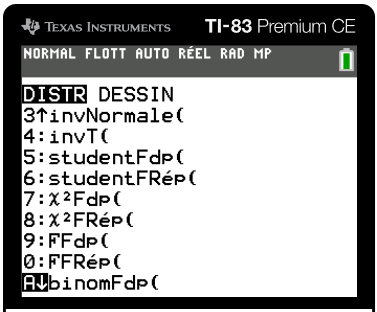
\includegraphics[width=0.27\linewidth]{ti01}\hfill 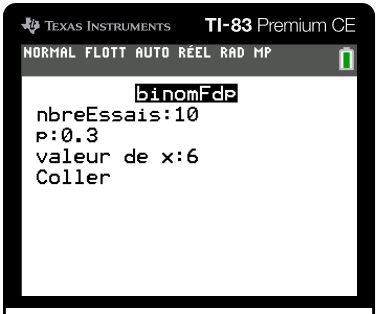
\includegraphics[width=0.27\linewidth]{ti02} \hfill 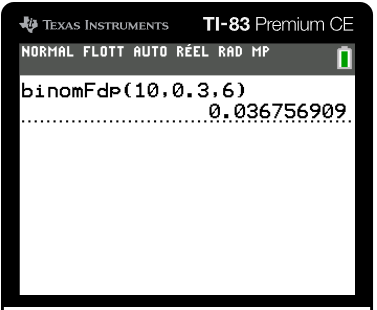
\includegraphics[width=0.27\linewidth]{ti03}

\textbf{Numworks} : Sélectionner \textbf{Probabilités} sur l'écran d'accueil, puis Binomiale. Entrer alors les valeurs des paramètres $n$ et $p$ puis valider.\\
Vous pouvez calculer des probabilités de la forme $\mathbb{P}(X\leqslant k)$, $\mathbb{P}(a\leqslant X \leqslant b)$, $\mathbb{P}(X \geqslant k)$ et $\mathbb{P}(X=k)$ en sélectionnant l'icône en haut à gauche de l'écran.

\vskip5pt

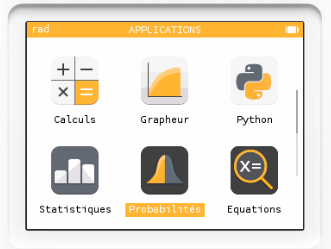
\includegraphics[width=0.23\linewidth]{num01}\hfill 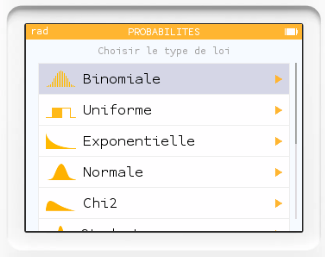
\includegraphics[width=0.23\linewidth]{num02}\hfill 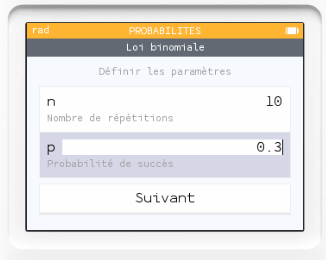
\includegraphics[width=0.23\linewidth]{num03} \hfill 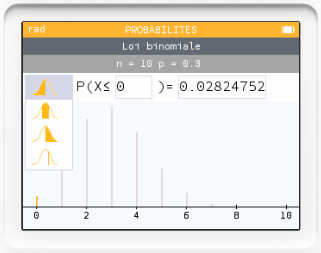
\includegraphics[width=0.23\linewidth]{num05}

\textbf{Casio Graph} : Dans le menu principal, sélectionner \textbf{STAT}. Appuyer ensuite sur \textbf{F5 [DIST]} puis \textbf{F5 [BINM]}.\\
Pour le calcul de $\mathbb{P}(X=k)$, appuyer sur \textbf{F1 [Bpd]}. Pour le calcul de $\mathbb{P}(X \leqslant k)$, appuyer sur \textbf{F2 [Bcd]}.\\
Sur l'écran suivant, placer le curseur sur \textbf{Data} et appuyer sur \textbf{F2 [Var]}. Renseigner alors les valeurs des paramètres de la loi binomiale et les valeurs de $k$.

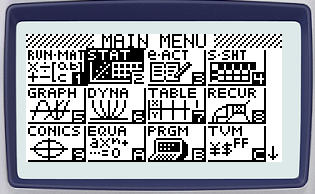
\includegraphics[width=0.23\linewidth]{casio01}\hfill 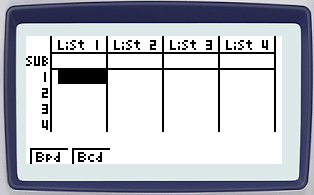
\includegraphics[width=0.23\linewidth]{casio04}\hfill 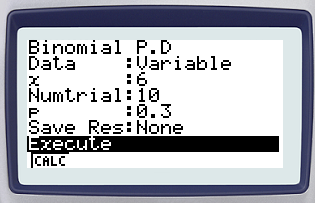
\includegraphics[width=0.23\linewidth]{casio05} \hfill 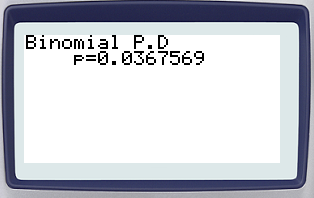
\includegraphics[width=0.23\linewidth]{casio06}


\subsubsection{Espérance, variance, écart-type}

\begin{proposition}Soit $X$ une variable aléatoire qui suit une loi binomiale $\mathcal{B}(n,p)$. L'espérance, la variance et l'écart-type de $X$ valent respectivement \[E[X]=np, \quad Var(X)=np(1-p), \quad \sigma(X)=\sqrt{np(1-p)}\]\end{proposition}

\begin{example}Un élève répond au hasard et de manière indépendante à un QCM de 20 questions. Chaque question laisse le choix entre 4 propositions dont une seule est correcte.

On note $X$ le nombre de bonnes réponses de l'élève. $X$ désigne donc le nombre de succès (bonnes réponses) d'un schéma de Bernoulli à 20 épreuves, chaque épreuve ayant une probabilité de succès de $\dfrac{1}{4}$. $X$ suit donc une loi binomiale $\mathcal{B}\left(20,\dfrac{1}{4}\right)$.

Ainsi, $E[X]=20 \times \dfrac{1}{4}=5$. L'élève peut espérer avoir 5 bonnes réponses.\end{example}






\end{document}